% \documentclass[smaller,handout]{beamer}

\def\bmode{2} % Mode 0 for presentation, mode 1 for a handout with notes, mode 2 for handout without notes
\if 0\bmode
\documentclass[smaller]{beamer}
\else \if 1\bmode
\immediate\write18{pdflatex -jobname=\jobname-Notes-Handout\space\jobname}
\documentclass[smaller,handout]{beamer}
\usepackage{handoutWithNotes}
\pgfpagesuselayout{2 on 1 with notes}[letterpaper, landscape, border shrink=4mm]
\else \if 2\bmode
\immediate\write18{pdflatex -jobname=\jobname-Handout\space\jobname}
\documentclass[smaller,handout]{beamer}
\fi
\fi
\fi


% \documentclass[smaller,handout
% ]{beamer}
%\usepackage{etex}
%\newcommand{\num}{6{} }

% \usetheme[
%   outer/progressbar=foot,
%   outer/numbering=counter,
%  block=fillFF
% ]{metropolis}

%\useoutertheme{metropolis}

\usetheme{Madrid}
\useoutertheme[subsection=false]{miniframes} % Alternatively: miniframes, infolines, split
\useinnertheme{circles}
\usecolortheme{seahorse}

\usepackage[backend=biber,style=authoryear,maxcitenames=2,maxbibnames=99,safeinputenc,url=false,
eprint=false]{biblatex}
\addbibresource{bib/references.bib}
\AtEveryCitekey{\iffootnote{{\tiny}\tiny}{\tiny}}

%\usepackage{pgfpages}
%\setbeameroption{hide notes} % Only slides
%\setbeameroption{show only notes} % Only notes
%\setbeameroption{hide notes} % Only notes
%\setbeameroption{show notes on second screen=right} % Both

% \usepackage[sfdefault]{Fira Sans}

% \setsansfont[BoldFont={Fira Sans}]{Fira Sans Light}
% \setmonofont{Fira Mono}

%\usepackage{fira}
%\setsansfont{Fira}
%\setmonofont{Fira Mono}
% To give a presentation with the Skim reader (http://skim-app.sourceforge.net) on OSX so
% that you see the notes on your laptop and the slides on the projector, do the following:
% 
% 1. Generate just the presentation (hide notes) and save to slides.pdf
% 2. Generate onlt the notes (show only nodes) and save to notes.pdf
% 3. With Skim open both slides.pdf and notes.pdf
% 4. Click on slides.pdf to bring it to front.
% 5. In Skim, under "View -> Presentation Option -> Synhcronized Noted Document"
%    select notes.pdf.
% 6. Now as you move around in slides.pdf the notes.pdf file will follow you.
% 7. Arrange windows so that notes.pdf is in full screen mode on your laptop
%    and slides.pdf is in presentation mode on the projector.

% Give a slight yellow tint to the notes page
%\setbeamertemplate{note page}{\pagecolor{yellow!5}\insertnote}\usepackage{palatino}


%\usetheme{metropolis}
%\usecolortheme{beaver}
%\usepackage{xcolor}
\definecolor{darkcandyapplered}{HTML}{A40000}
\definecolor{lightcandyapplered}{HTML}{e74c3c}

%\setbeamercolor{title}{fg=darkcandyapplered}
%\setbeamercolor{frametitle}{bg=darkcandyapplered!80!black!90!white}
%\setbeamertemplate{frametitle}{\bf\insertframetitle}
%\setbeamercolor{footnote mark}{fg=darkcandyapplered}
%\setbeamercolor{footnote}{fg=darkcandyapplered!70}
%\Raggedbottom
%\setbeamerfont{page number in head/foot}{size=\tiny}
%\usepackage[tracking]{microtype}


\setbeamertemplate{frametitle}{%
    \nointerlineskip%
    \begin{beamercolorbox}[wd=\paperwidth,ht=2.0ex,dp=0.6ex]{frametitle}
        \hspace*{1ex}\insertframetitle%
    \end{beamercolorbox}%
}



\setbeamerfont{caption}{size=\footnotesize}
\setbeamercolor{caption name}{fg=darkcandyapplered}


%\usepackage[sc,osf]{mathpazo}   % With old-style figures and real smallcaps.
%\linespread{1.025}              % Palatino leads a little more leading

% Euler for math and numbers
%\usepackage[euler-digits,small]{eulervm}
%\AtBeginDocument{\renewcommand{\hbar}{\hslash}}
\usepackage{graphicx,multirow,paralist,booktabs}


%\mode<presentation> { \setbeamercovered{transparent} }

\setbeamertemplate{navigation symbols}{}
\makeatletter
\def\beamerorig@set@color{%
  \pdfliteral{\current@color}%
  \aftergroup\reset@color
}
\def\beamerorig@reset@color{\pdfliteral{\current@color}}
\makeatother

%=== GRAPHICS PATH ===========
\graphicspath{{./m4-images/}}
% Marginpar width
%Marginpar width
%\setlength{\marginparsep}{.02in}


%% Captions
% \usepackage{caption}
% \captionsetup{
%   labelsep=quad,
%   justification=raggedright,
%   labelfont=sc
% }

%AMS-TeX packages

\usepackage{amssymb,amsmath,amsthm} 
\usepackage{bm}
\usepackage{color}

\usepackage{hyperref,enumerate}
\usepackage{minitoc,array}


%https://tex.stackexchange.com/a/31370/2269
\usepackage{mathtools,cancel}

\renewcommand{\CancelColor}{\color{red}} %change cancel color to red

\makeatletter
\let\my@cancelto\cancelto %copy over the original cancelto command
\newcommand<>{\cancelto}[2]{\alt#3{\my@cancelto{#1}{#2}}{\mathrlap{#2}\phantom{\my@cancelto{#1}{#2}}}}
% redefine the cancelto command, using \phantom to assure that the
% result doesn't wiggle up and down with and without the arrow
\makeatother


\definecolor{slblue}{rgb}{0,.3,.62}
\hypersetup{
    colorlinks,%
    citecolor=blue,%
    filecolor=blue,%
    linkcolor=blue,
    urlcolor=slblue
}

%%% TIKZ
\usepackage{animate}
\usepackage{tikz}
\usepackage{pgfplots}
\usepackage{pgfplotstable}
\usepackage{pgfgantt}
\usepackage{tikzsymbols}
\pgfplotsset{compat=newest}
\usepgfplotslibrary{groupplots,fillbetween}

\usetikzlibrary{arrows,shapes,positioning,shapes.geometric}
\usetikzlibrary{decorations.markings}
\usetikzlibrary{shadows,automata}
\usetikzlibrary{patterns,matrix}
\usetikzlibrary{trees,mindmap,backgrounds}
%\usetikzlibrary{circuits.ee.IEC}
\usetikzlibrary{decorations.text}
% For Sagnac Picture
\usetikzlibrary{%
    decorations.pathreplacing,%
    decorations.pathmorphing%
}
\tikzset{no shadows/.style={general shadow/.style=}}
%
%\usepackage{paralist}



%%% FORMAT PYTHON CODE
%\usepackage{listings}
% Default fixed font does not support bold face
\DeclareFixedFont{\ttb}{T1}{txtt}{bx}{n}{8} % for bold
\DeclareFixedFont{\ttm}{T1}{txtt}{m}{n}{8}  % for normal

% Custom colors
\definecolor{deepblue}{rgb}{0,0,0.5}
\definecolor{deepred}{rgb}{0.6,0,0}
\definecolor{deepgreen}{rgb}{0,0.5,0}

%\usepackage{listings}

% Python style for highlighting
% \newcommand\pythonstyle{\lstset{
% language=Python,
% basicstyle=\footnotesize\ttm,
% otherkeywords={self},             % Add keywords here
% keywordstyle=\footnotesize\ttb\color{deepblue},
% emph={MyClass,__init__},          % Custom highlighting
% emphstyle=\footnotesize\ttb\color{deepred},    % Custom highlighting style
% stringstyle=\color{deepgreen},
% frame=tb,                         % Any extra options here
    % showstringspaces=false            % 
% }}

% % Python environment
% \lstnewenvironment{python}[1][]
% {
% \pythonstyle
% \lstset{#1}
% }
% {}

% % Python for external files
% \newcommand\pythonexternal[2][]{{
% \pythonstyle
% \lstinputlisting[#1]{#2}}}

% Python for inline
% 
% \newcommand\pythoninline[1]{{\pythonstyle\lstinline!#1!}}


\newcommand{\osn}{\oldstylenums}
\newcommand{\dg}{^{\circ}}
\newcommand{\lt}{\left}
\newcommand{\rt}{\right}
\newcommand{\pt}{\phantom}
\newcommand{\tf}{\therefore}
\newcommand{\?}{\stackrel{?}{=}}
\newcommand{\fr}{\frac}
\newcommand{\dfr}{\dfrac}
\newcommand{\ul}{\underline}
\newcommand{\tn}{\tabularnewline}
\newcommand{\nl}{\newline}
\newcommand\relph[1]{\mathrel{\phantom{#1}}}
\newcommand{\cm}{\checkmark}
\newcommand{\ol}{\overline}
\newcommand{\rd}{\color{red}}
\newcommand{\bl}{\color{blue}}
\newcommand{\pl}{\color{purple}}
\newcommand{\og}{\color{orange!90!black}}
\newcommand{\gr}{\color{green!40!black}}
\newcommand{\nin}{\noindent}
\newcommand{\la}{\lambda}
\renewcommand{\th}{\theta}
\newcommand{\al}{\alpha}
\newcommand{\G}{\Gamma}
\newcommand*\circled[1]{\tikz[baseline=(char.base)]{
            \node[shape=circle,draw,thick,inner sep=1pt] (char) {\small #1};}}

\newcommand{\bc}{\begin{compactenum}[\quad--]}
\newcommand{\ec}{\end{compactenum}}

\newcommand{\p}{\partial}
\newcommand{\pd}[2]{\frac{\partial{#1}}{\partial{#2}}}
\newcommand{\dpd}[2]{\dfrac{\partial{#1}}{\partial{#2}}}
\newcommand{\pdd}[2]{\frac{\partial^2{#1}}{\partial{#2}^2}}
\newcommand{\nmfr}[3]{\Phi\left(\frac{{#1} - {#2}}{#3}\right)}


\pgfmathdeclarefunction{poiss}{1}{%
  \pgfmathparse{(#1^x)*exp(-#1)/(x!)}%
  }

\pgfmathdeclarefunction{gauss}{2}{%
  \pgfmathparse{1/(#2*sqrt(2*pi))*exp(-((x-#1)^2)/(2*#2^2))}%
}

\pgfmathdeclarefunction{expo}{2}{%
  \pgfmathparse{#1*exp(-#1*#2)}%
}

\pgfmathdeclarefunction{expocdf}{2}{%
  \pgfmathparse{1 -exp(-#1*#2)}%
}

\makeatletter
\long\def\ifnodedefined#1#2#3{%
    \@ifundefined{pgf@sh@ns@#1}{#3}{#2}%
}

\pgfplotsset{
    discontinuous/.style={
    scatter,
    scatter/@pre marker code/.code={
        \ifnodedefined{marker}{
            \pgfpointdiff{\pgfpointanchor{marker}{center}}%
             {\pgfpoint{0}{0}}%
             \ifdim\pgf@y>0pt
                \tikzset{options/.style={mark=*, fill=white}}
                \draw [densely dashed] (marker-|0,0) -- (0,0);
                \draw plot [mark=*] coordinates {(marker-|0,0)};
             \else
                \tikzset{options/.style={mark=none}}
             \fi
        }{
            \tikzset{options/.style={mark=none}}        
        }
        \coordinate (marker) at (0,0);
        \begin{scope}[options]
    },
    scatter/@post marker code/.code={\end{scope}}
    }
}

\makeatother

\renewcommand{\arraystretch}{1.5}
%%%%%%%%%%%%%%%%%%%%%%%%%%%%%%%%%%%%%%%%%%%%%%%%%%%
%%%%%%%%%%%%%%%%%%%%%%%%%%%%%%%%%%%%%%%%%%%%%%%%%%%

\title[CEE 260/MIE 273 M4a: Point Estimates and Sampling Variability]{{\normalsize CEE 260/MIE 273: Probability and Statistics in Civil Engineering} \\
Lecture M4a: Point Estimates, Sampling Variability and Central Limit Theorem}
\date[\today]{\footnotesize \today}
\author{{\bf Jimi Oke}}
\institute[UMass Amherst]{
  \begin{tikzpicture}[baseline=(current bounding box.center)]
    \node[anchor=base] at (-7,0) (its) {
\includegraphics[scale=.3]{UMassEngineering_vert}} ;
  \end{tikzpicture}
}



%https://tex.stackexchange.com/questions/55806/mindmap-tikzpicture-in-beamer-reveal-step-by-step
  % \tikzset{
  %   invisible/.style={opacity=0},
  %   visible on/.style={alt={#1{}{invisible}}},
  %   alt/.code args={<#1>#2#3}{%
  %     \alt<#1>{\pgfkeysalso{#2}}{\pgfkeysalso{#3}} % \pgfkeysalso doesn't change the path
  %   },
  % }


\usepackage{listings}

\lstset{language=matlab,
                basicstyle=\scriptsize\ttfamily,
                keywordstyle=\color{blue}\ttfamily,
                stringstyle=\color{blue}\ttfamily,
                commentstyle=\color{gray}\ttfamily,
                morecomment=[l][\color{gray}]{\#}
              }
         
\begin{document}

\maketitle




\begin{frame}
  \frametitle{Outline}
  \tableofcontents
\end{frame}



\section{Statistical inference}

\begin{frame}
  \frametitle{Statistical inference}\pause

  \begin{minipage}[]{.45\linewidth}
    To develop probabilistic models from observational data, we need to \textit{estimate} the statistical parameters and probabilities of the distributions.

    \bigskip
    
  \begin{itemize}[<+->]
  \item In most applications, the true population is unknown
    \medskip
    
  \item Estimates are obtained from representative {\bf samples}
    
  \end{itemize}    
\end{minipage}\pause\quad\quad
\begin{minipage}[]{.45\linewidth}
  \begin{center}
  \only<5->{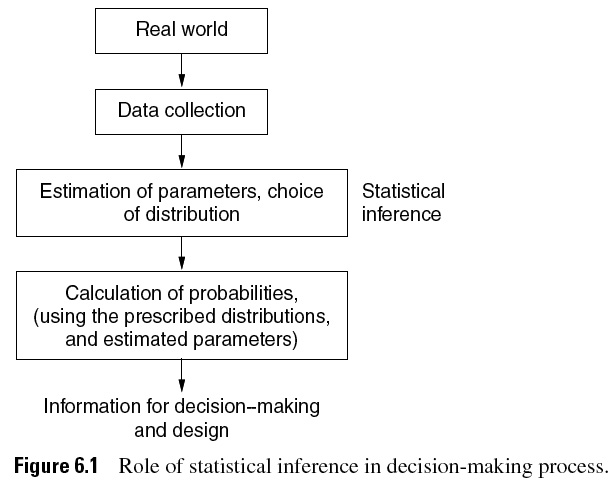
\includegraphics[width=.8\textwidth,  trim={0 1cm 0 0}, clip]{06_01}}
\end{center}
\end{minipage}
\end{frame}


\begin{frame}
  \frametitle{Role of sampling in statistical inference}
  \begin{center}
  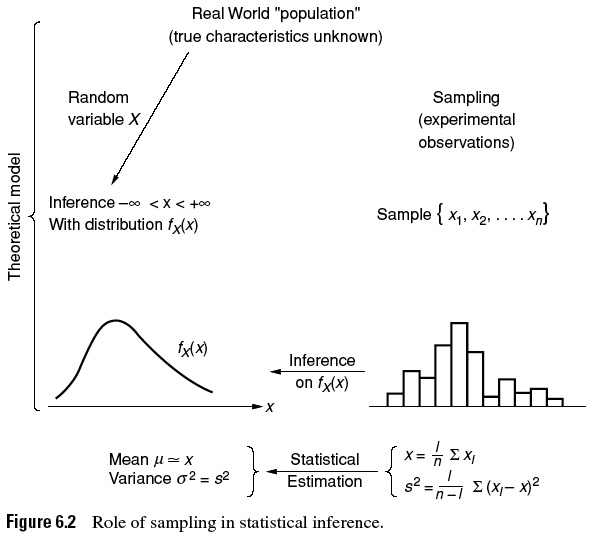
\includegraphics[width=.7\textwidth, trim={0 1cm 0 0}, clip]{06_02}
\end{center}

\end{frame}

\begin{frame}
  \frametitle{Statistical inference}
  \pause

  This module (M4) covers concepts in statistical inference: \pause
  \begin{itemize}[<+->]
  \item Point estimates and sampling variability (M4a; today)
  \item Confidence intervals for a proportion (M4b)
  \item Hypothesis testing for a proportion (M4c)
  \end{itemize}
\end{frame}

\section{Point estimation}
\begin{frame}
  \frametitle{Point estimates}
  \begin{definition}
    A \textbf{point estimate} of a parameter $\theta$ (e.g.\ proportion $p$, or mean value $\mu$) is a single number that can be regarded as a sensible value for
    $\theta$ and is obtained by computing the value of a suitable statistic from given sample data. \pause The selected
    statistic is the \textbf{point estimator} of $\theta$.
  \end{definition}
  \pause
  \begin{block}{Notation}\pause
    \begin{itemize} 
    \item $\hat\Theta$: point estimator (pronounced {\it theta hat}) \pause
    \item $\hat\theta$: point estimate\pause
      \begin{equation}
        \label{eq:3}
        \hat\theta  = \theta + \text{ estimation error}\pause
      \end{equation}
    \item A hat can be placed on the actual statistic estimated for clarity, e.g. \pause
      \begin{equation*}
        \hat{p} = \ol{X}
      \end{equation*}
    \end{itemize}
  \end{block}
\end{frame}

\begin{frame}
  \frametitle{Properties of point estimators}
   Desired properties of a point estimator:\pause
  \begin{itemize}[<+->]
  \item Unbiasedness
  \item Consistency
  \item Efficiency
  \item Sufficiency
  \end{itemize}
\end{frame}

\begin{frame}
  \frametitle{Desired properties of point estimators}
  \begin{block}{Unbiasedness}
    An estimator is \textit{unbiased} if its expected value is equal to the true value of the parameter it estimates:\pause
    \begin{equation}
      \label{eq:1}
      \mathbb{E}(\hat\theta) = \theta \pause \quad \text{(if $\hat\theta$ is unbiased)}
    \end{equation}
    \pause
    Thus, the \textbf{\rd bias} is given by:\pause
    \begin{equation}
      \label{eq:2}\rd
     \text{Bias}_{\hat\theta} = \pause  \mathbb{E}(\hat\theta) - \theta
    \end{equation}
  \end{block}
  \pause

  \begin{block}{Consistency}\pause
    An estimator is consistent if $\hat\theta \to \theta$ as $n\to \infty$,\pause i.e. the estimation error should decrease with increasing sample size.
  \end{block}

\end{frame}

\begin{frame}
  \frametitle{Desired properties of point estimators}
  \begin{block}{Efficiency}\pause
    The efficiency of an estimator is defined by how small its variance is.
  \end{block}
  \pause

  \begin{block}{Sufficiency}\pause
    A sufficient estimator uses all the relevant information in a given sample in its estimation.
  \end{block}
  \pause

  \bigskip
  
  In many applications, \alert{efficiency} (low variance)  and \alert{unbiasedness} (low bias)  are the most important properties of an estimator.
\end{frame}



% \begin{frame}
%   \frametitle{Mean squared error of an estimator}
%   \pause

%   The mean squared error (MSE) of an estimator is given by:

%   \pause

%   \begin{equation}

\begin{frame}
  \frametitle{Bias vs.\  variance}

  \pause

  \begin{center}
    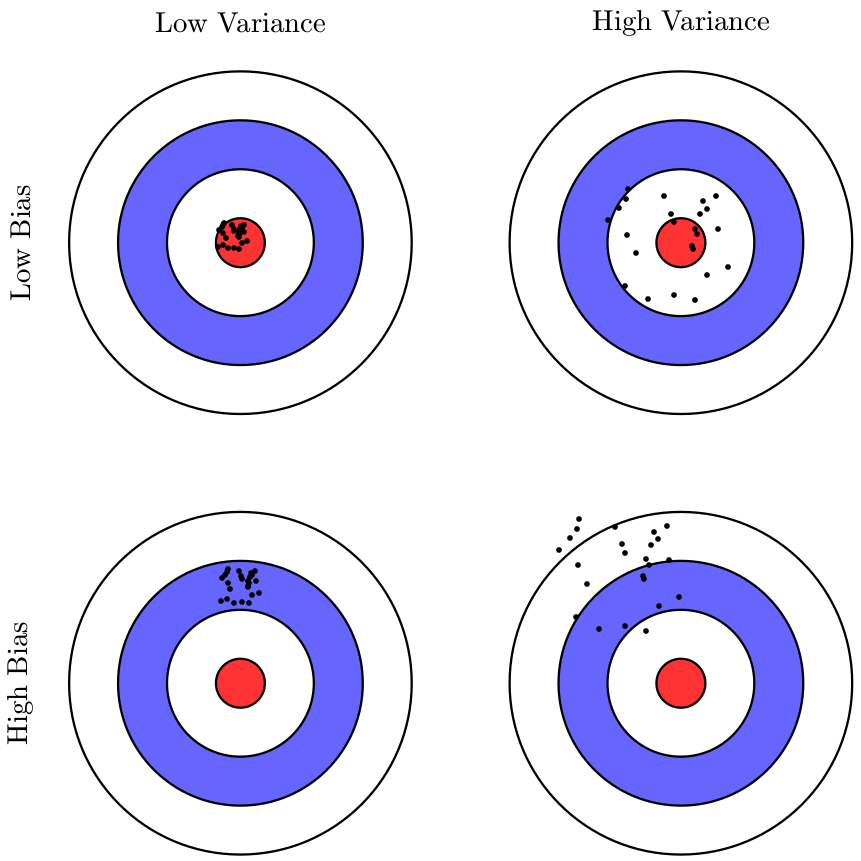
\includegraphics[width=.5\textwidth]{bivar}
  \end{center}
% \begin{pspicture}(3.45,3.45)
%   \target(0.25,0)
%   \target(2.05,0)
%   \target(0.25,1.8)
%   \target(2.05,1.8)
%   \dots[0.12](0.95,1.1)
%   \dots[0.1](0.92,2.53)
%   \dots[0.3](2.5,1.15)
%   \dots[0.3](2.7,2.5)
%   \rput{90}(0.05,0.7){High Bias}
%   \rput{90}(0.05,2.5){Low Bias}
%   \rput(0.95,3.4){Low Variance}
%   \rput(2.75,3.4){High Variance}
% \end{pspicture}

{\footnotesize Image source: \url{https://tex.stackexchange.com/a/307285/2269}}
\end{frame}


\section{Method of moments}
\begin{frame}
  \frametitle{Sample moments}\pause
  \begin{itemize}[<+->]
  \item The moments of a random variable are its key descriptors.
  \item Parameters of the distribution of a random variable are usually related to the {\bl first} and {\gr second}
    moments \pause ({\bl mean} and \pause {\gr variance}, respectively)
  \end{itemize}

  \pause
  Given a sample $x_1, x_2, \ldots, x_n$, the point estimates of the population mean $\mu$ and variance $\sigma^2$ are:
  \pause
  
  \begin{block}{Sample mean}\pause
    \begin{equation}
      \label{eq:4}
      \ol{x} = \fr1n\sum_{i=1}^n x_i 
    \end{equation}
  \end{block}
  \pause
  \begin{block}{Sample variance}\pause
    \begin{equation}
      \label{eq:5}
      s^2 = \fr{1}{n-1}\sum_{i=1}^n(x_i - \ol{x})^2      
    \end{equation}
  \end{block}
\end{frame}

\begin{frame}
  \frametitle{Unbiasedness of $s^2$}
  From Equation \eqref{eq:5}, you can show (as an exercise) that:
  \begin{equation}
    \label{eq:6}
    s^2 = \fr{1}{n-1}\lt[ \sum_{i=1}^nx_i^2 - n \ol{x}^2\rt]
  \end{equation}
  You may be wondering why the sample variance is not just the average of the sum of squared deviations from the sample mean. \pause But
   \begin{eqnarray}
      \label{eq:7}
     s^{2} \pause =  E\lt( \fr{1}{n-1}\sum_{i=1}^n(x_i - \ol{x})^2 \rt) &=& \pause \sigma^2 \\\pause
     \hat\sigma^{2} \pause = E\lt( \fr{1}{n}\sum_{i=1}^n(x_i - \ol{x})^2 \rt) &=& \pause \fr{n-1}{n}\sigma^2 
   \end{eqnarray}
   \pause The second estimator is biased ($-\fr{\sigma^2}{n}$) and underestimates $\sigma^2$. 
\end{frame}

\begin{frame}
  \frametitle{Sample mean and variance}
  \begin{exampleblock}{Example 1: Elastic modulus of alloys}\pause
    The elastic modulus (GPa) of a sample of alloy specimens from a die-casting process is:
    \[X = 44.2, 43.9, 44.7, 44.2, 44.0, 43.8, 44.6, 43.1\]
    \pause
    \begin{enumerate}[(a)]
    \item Estimate the population mean using the estimator $\ol{x}$ (sample mean)\pause
    \item Estimate the population variance using the estimator $s^2$ (sample variance)\pause
    \item Now, estimate the variance replacing the denominator $(n-1)$ with $n$ in the estimator $s^2$. What do you notice?
    \end{enumerate}
  \end{exampleblock}
\end{frame}

\begin{frame}
  \frametitle{Sample mean and variance}
  \begin{exampleblock}{Example 1: Elastic modulus of alloys (cont.)}\pause
    $X = 44.2, 43.9, 44.7, 44.2, 44.0, 43.8, 44.6, 43.1$ \pause
    
    \begin{enumerate}[(a)]
    \item $\hat\mu = \pause \ol{x} = \pause \fr18\sum_{i=1}^8x_i \pause \approx  \boxed{44.063}$ \pause
      \bigskip
      
    \item $s^2 = \pause \fr17 \lt[\sum_{i=1}^8 x_i^2 - 8(44.063^2)\rt] \pause \approx \boxed{0.251}$ \pause
      \bigskip
      
      
    \item Biased estimate of $\sigma^2$:\\ \pause
      $\hat\sigma^{2} = \pause \fr18 \lt[\sum_{i=1}^8 x_i^2 - 8(44.063^2)\rt] \pause = \fr78\lt(0.251\rt) \pause = \boxed{0.220}$
      \pause

      $\hat\sigma^{2}$ underestimates $\sigma^{2}$ by $0.031$ squared units.
    \end{enumerate}
  \end{exampleblock}
\end{frame}


 \section{Variability and CLT}
\begin{frame}
  \frametitle{Variability of a point estimate}
  \pause
  
  \begin{exampleblock}{Example 2: Solar energy expansion}
    Suppose the proportion of American adults who support the expansion of solar energy is $p = 0.88$, which is our
    parameter of interest. Develop a simulation to investigate how the sample proportion $\hat{p}$ behaves compared to the true population proportion $p$:

    \pause
    
    \begin{enumerate}[\bf (a)]
    \item  Create a set of a large number of entries (e.g.\ 300 million) where 88\% are in support and 12\% are not.\pause
    \item Sample $n=1000$ entries without replacement \pause
    \item Plot the histogram of the sampling distribution of $\hat{p}$
    \item Compute the sample mean $x_{\hat{p}}$
    \item Compute the standard deviation $s_{\hat{p}}$ (called the \textbf{standard error} $SE_{\hat{p}}$).
    \item Investigate what happens as $n$ increases.
    \end{enumerate}
  \end{exampleblock}
  
\end{frame}



 \begin{frame}
  \frametitle{The Central Limit Theorem (CLT)}
  
  \begin{theorem}%{Central Limit Theorem (CLT)}
    Let $X_1, X_2,\ldots,X_n$ be a random sample from a distribution with mean
    $\mu$ and variance $\sigma^2$. If $n$ is sufficiently large,  then the
    sample mean $\ol{X}$ has approximately a normal distribution with
    $\mu_{\ol{X}} = \mu$ and $\sigma_{\ol{X}}^2 = \sigma^2/n$; and the sample total
    ($S_{n} = X_1 + X_2 + \ldots + X_n$) has approximately a normal distribution
    with
    \begin{eqnarray}
      \mu_S &= n\mu \\\pause
      \sigma^2_S &= n\sigma^2
    \end{eqnarray}
  \end{theorem}
  \pause
  Implications:
  \begin{itemize}[<+->]
  \item The sum of a \textbf{large number} of random components approaches a \textbf{normal/Gaussian distribution}
  \item The product of large number of random components approaches the lognormal distribution
  \end{itemize}
\end{frame}

\begin{frame}
  \frametitle{Central limit theorem (cont.)}
  \pause
  \begin{block}{Sample mean}
    \pause
    \begin{equation}
      \ol{X} \pause = \fr{X_{1} + X_{2} + \cdots + X_{n}}{n} 
    \end{equation}
  \end{block}

  \pause

  \begin{block}{Sum of sample observations}
    \pause
    \begin{equation}
      S_{n} = \pause X_{1} + X_{2} + \cdots + X_{n}
    \end{equation}
  \end{block}
  \pause

  If $n$ is sufficiently large for \textbf{any} sample: \pause
  \begin{eqnarray}
    \ol{X} &\sim& \pause \mathcal{N}\lt(\mu, \fr{\sigma^{2}}{n}\rt) \\\pause
    S_{n} &\sim& \pause \mathcal{N}(n\mu, n\sigma^{2}) 
  \end{eqnarray}
  \pause
  Note that the quantity {\rd $\sqrt{\fr{\sigma^{2}}{n}} = \pause \fr{\sigma}{\sqrt{n}}$}
  is also known as the {\rd \textbf{sampling error} (SE)} \pause
  or the {\rd \textbf{standard error of the mean} (SEM)}
\end{frame}

\begin{frame}
  \frametitle{Sample proportion and the CLT}
  If the observations in a given sample are a Bernoulli sequence with a constant proportion (or probability) $p$, then
  if $n$ is large, the sample proportion $\hat p$ follows a normal distribution (according to the CLT):

  \begin{block}{}
    \begin{equation}
    \hat p \sim \mathcal{N}(\mu_{\hat p}, SE^{2}_{\hat p}) = \mathcal{N}\lt( p, \fr{p(1-p)}{n}\rt)
  \end{equation}
  where
  \begin{eqnarray*}
  \text{Sample mean proportion: }  \mu_{\hat p} &=& p \\ \pause
    \text{Sampling error/standard error of $\hat p$: }    SE_{\hat p} &=& \sqrt{\fr{p (1- p)}{n}}
  \end{eqnarray*}
\end{block}

One rule of thumb for determining whether $n$ is large enough is to check that both $np$ and $n(1-p)$ are $\ge 10$ (also known as the success-failure condition).
\end{frame}


\begin{frame}
  \frametitle{CLT application: sample proportion}
  \pause

  \begin{exampleblock}{Example 3: Solar energy expansion (CLT)}
    Suppose the proportion of American adults who support the expansion of solar energy is $p = 0.88$, which is our
    parameter of interest. \pause If we were to take a poll of 1000 American adults on this topic, the estimate would not be
    perfect, but how close might we expect the sample proportion in the poll would be to 88\%? 

    \pause
    
    \begin{enumerate}[\bf (a)]
    \item     According to the CLT, what is the distribution of $\hat p$?
    \item According to the CLT, what are $\mu_{\hat p}$ and $SE_{\hat p}$, respectively? 
    \end{enumerate}
  \end{exampleblock}
\end{frame}

\begin{frame}
  \frametitle{CLT application: sample proportion (cont.)}
  \pause

  \begin{exampleblock}{Example 3: Solar energy expansion (CLT)}
    \begin{enumerate}[\bf (a)]
    \item First, we note that the response of each American adult in the entire population is part of a Bernoulli
      sequence with $p=0.88$.  According to the CLT, the distribution of $\hat p$ (the mean proportion
      based on the sample) is normal/Gaussian. We can denote this as:
      \begin{equation}
        \hat p \sim \mathcal{N}\lt(p, \fr{\sigma^{2}}{n}\rt) \text{ OR } \mathcal{N}\lt(\mu_{p}, \fr{\sigma^{2}_{p}}{n}\rt)
      \end{equation}
    \item $\mu_{\hat p} $ denotes the mean estimate of $p$, which is 0.88 (according to the CLT, the mean of the sample
      is the population mean if $n$ is large).\\

      $SE_{\hat p}$ denotes the sampling error, which is the the square root of the variance of the sample mean:
      $\sqrt{\sigma^{2}/n}$. Given that the sample is governed by the Binomial distribution with $\sigma^{2} = p(1-p)$. Thus:
      \begin{eqnarray*}
        SE_{\hat p}^{2} &=& \fr{\sigma^{2}}{n} = \fr{p(1-p)}{n} =  \fr{0.88(0.12)}{1000} \\
        SE_{\hat p} &=& \sqrt{ \fr{0.88(0.12)}{1000}} = \boxed{0.01}
      \end{eqnarray*}
    \end{enumerate}
  \end{exampleblock}
\end{frame}

\begin{frame}
  \frametitle{Success-failure condition}
  \pause
  In the case of a proportion $p$, the CLT holds only if: \pause
  \begin{itemize}
  \item The observations are independent (i.e.\ random) \pause
  \item The sample size $n$ is \textbf{sufficiently large}
  \end{itemize}
  \pause
  The second condition is typically observed via the \textbf{success-failure condition}, i.e.:\pause
  \begin{eqnarray}
    np &\geq& 10 \\\pause
    n(1-p) &\geq& 10
  \end{eqnarray}
\end{frame}

\begin{frame}
  \frametitle{Another application of the CLT}
  \begin{exampleblock}{Example 4: Mean batch weight} %4.24
    A certain brand of cement is shipped in batches of 40 bags. Previous records
    indicate the weight of a randomly selected bag of this brand has a mean of
    2.5 kg and an SD of 0.1 kg. The exact distribution is unknown.\pause
    \begin{enumerate}[(a)]
    \item What is the mean weight of one batch of this brand of cement?\pause
    \item If the shipping company charges an overweight fee if a batch exceeds
      the mean batch weight by more than 1 kg, what is the probability that a
      batch will be charged?
    \end{enumerate}
  \end{exampleblock}
\end{frame}


\begin{frame}
  \frametitle{Another application of the CLT}
  \begin{exampleblock}{Example 4: Mean batch weight (cont.)}\pause
    Let $B$ be the total weight of one batch. \pause
    \begin{enumerate}[(a)]
    \item The mean weight of one batch is thus\pause
      \begin{equation}
        \label{eq:42}
        \mu_B = \pause 40 \times 2.5 \pause = 100 \text{ kg}
      \end{equation}
      \pause
    \item By the CLT, $B$ is approximately normal with $\mu_B = 100$ and $\sigma^2_B = 40(0.1)^2$.\pause
      The probability a batch will be charged is:\pause
      \begin{eqnarray*}
        P(B > 101) &=& 1 - \nmfr{101}{100}{0.1\sqrt{40}} \\\pause
                   &=& 1 - \Phi(1.581) \\\pause
                   &=& 1- 0.9431 \pause \approx \boxed{5.69\%}
      \end{eqnarray*}
    \end{enumerate}
  \end{exampleblock}
\end{frame}

\section{Outlook}
\begin{frame}
  \frametitle{Summary}
  \begin{itemize}
  \item Desired properties of point estimates: unbiasedness and efficiency
  \item Distribution of sample proportions (or other parameters) is called a sampling distribution
  \item When $n$ is sufficiently large and observations are independent, the sample proportion (or other parameter) follows a normal distribution
    \item The success-failure condition can be used to determine if $n$ is large enough for the CLT to hold (for a sample proportion)
  \end{itemize}
\end{frame}

\appendix
\section{Introduction to simulation}

\begin{frame}
  \frametitle{Simulation}

  \pause

  Simulation is the process of representing (modeling) a hypothetical process using a compute in order to compute or
  evaluate outcomes absent of real-life experimentation. \pause

  \medskip

  \begin{block}{Uses of simulation}
    \pause

    \begin{itemize}
    \item Estimating probabilities \pause
    \item Estimating statistical parameters for a given population, such as mean, median and variance
    \item Finding the bias (difference between true and estimated value) of a given parameter
    \item Synthesizing data
    \item Conducting experiments
    \end{itemize}
  \end{block}
\end{frame}

\begin{frame}
  \frametitle{Example 4: Estimating probability via simulation}
  \pause

  \begin{exampleblock}{}
    A motorist is driving at the posted maximum speed along a stretch of road. The
    probability that the motorist approaches a red light at the first intersection (A) is 0.4. The probability
    that the motorist encounters a red light \textit{again} at the next intersection (B) is 0.7. If the
    motorist does not encounter a red light at the first intersection (A), then the probability the
    motorist encounters a red light at the second intersection (B) is 0.2. If in a certain instance the motorist is observed
    to have encountered a red light at  intersection B, what is the probability the motorist encountered
    a red light at intersection A?

    \pause

    \begin{enumerate}[\bf(a)]
    \item First use Bayes' Theorem to compute the required probability. \pause Recall:\pause

      \begin{equation}
        P(A|B) = \pause \fr{P(B|A)P(A)}{P(B)} \pause = \fr{P(B|A)P(A)}{P(B|A)P(A) + P(B|\ol{A})P(\ol{A})}
      \end{equation}
      \pause
    \item Perform a simulation to estimate this probability.
    \end{enumerate}
\end{exampleblock}
\end{frame}

\begin{frame}
  \frametitle{Example 4: Estimating probability via simulation (cont.)}
  \begin{exampleblock}{Solution}
    \begin{enumerate}[\bf (a)]
    \item From the problem, we know that  $P(A) = 0.4$, $P(B|A) = 0.7$, $P(B|\ol{A}) = 0.2$. Thus,
      \begin{eqnarray*}
        P(A|B) &=& \fr{P(B|A)P(A)}{P(B|A)P(A) + P(B|\ol{A})P(\ol{A})} \\
               &=& \fr{0.7 (0.4)}{0.7 (0.4) + (0.2)( 1 - 0.4)} \\
               &=& \fr{0.28}{0.28 + 0.12} \\
               &=&  \boxed{0.7}
      \end{eqnarray*}

    \item For the simulation, see \texttt{M4\_matlab\_example4.m}
    \end{enumerate}
  \end{exampleblock}
\end{frame}
% \begin{frame}
%   \frametitle{Standard error}
%   \pause
  
%   Standard deviation of sample mean (\textbf{\bl known} population variance):

%   \pause
%   \begin{equation}
%     \label{eq:21}
%     \boxed{\sigma_{\ol{x}} = \fr{\sigma}{\sqrt{n}}}
%   \end{equation}
%   \pause

%   Standard deviation of sample mean (\textbf{\og unknown} population variance):
%   \pause
  
%   \begin{equation}
%     \label{eq:se}
%     \boxed{\sigma_{\ol{x}} = \fr{s}{\sqrt{n}}}
%   \end{equation}
%   \pause
%   Equation \eqref{eq:se} is also called the \textbf{\og standard error} of the mean \pause (SE)
% \end{frame}
 

%\begin{frame}[allowframebreaks]
%   \frametitle{References}
%   \AtNextBibliography{\scriptsize}
%   \setbeamertemplate{bibliography item}[text]
%   \printbibliography[heading=none]
  
% \end{frame}

%\printbibliography
\end{document}
%%% Local Variables:
%%% mode: latex
%%% TeX-master: t
%%% End:
